\documentclass[conference]{IEEEtran}
\usepackage[english]{babel}
\usepackage{latexsym}

\usepackage{blindtext}
\usepackage{cite}
\usepackage{amsmath,amssymb,amsfonts}
\usepackage{algorithmicx}
\usepackage{textcomp}
\usepackage{graphicx}
\usepackage{xcolor}
\usepackage{placeins}
% urls
\usepackage{hyperref}

% codesource listings
\usepackage{listings}
\usepackage{array}
\usepackage{microtype}
\usepackage{wrapfig}
\usepackage{enumitem}
\usepackage{fancyhdr}
\usepackage{lastpage}
\usepackage{subcaption}

\graphicspath{ {images/} }

\makeatletter
\newcommand{\linebreakand}{%
  \end{@IEEEauthorhalign}
  \hfill\mbox{}\par
  \mbox{}\hfill\begin{@IEEEauthorhalign}
}
\makeatother

\begin{document}

\lstset{breaklines=true}

\title{Implementation of Generative Adversarial Networks in HPCC Systems using GNN Bundle}

\author{\IEEEauthorblockN{Ambu Karthik}
\IEEEauthorblockA{Computer Science and Engineering\\
R. V. College of Engineering\\
Bengaluru, India\\
Email: ambukarthik.cs18@rvce.edu.in}
\and
\IEEEauthorblockN{Prof. Jyothi S.}
\IEEEauthorblockA{Computer Science and Engineering\\
R. V. College of Engineering\\
Bengaluru, India\\
Email: jyothis@rvce.edu.in}
\and
\IEEEauthorblockN{Dr. Shobha G.}
\IEEEauthorblockA{Computer Science and Engineering\\
R. V. College of Engineering\\
Bengaluru, India\\
Email: shobhag@rvce.edu.in}
\linebreakand
\IEEEauthorblockN{Roger Dev}
\IEEEauthorblockA{Sr. Architect, Machine Learning\\
Lexis Nexis Risk Solutions\\
Alpharetta, Georgia, United States\\
Email: Roger.Dev@lexisnexisrisk.com}
}

\maketitle

\begin{abstract}
HPCC Systems, an open source cluster computing platform for big data analytics consists of Generalized Neural Network bundle with a wide variety of features which can be used for various neural network applications. To enhance the functionality of the bundle, this paper proposes the design and development of Generative Adversarial Networks (GANs) on HPCC Systems platform using ECL, a declarative language on which HPCC Systems works. GANs have been developed on the HPCC Platform by defining the Generator and Discriminator models separately, and training them by batches in the same epoch. In order to make sure that they train as adversaries, a certain weights transfer methodology was implemented. MNIST dataset which has been used to test the proposed approach has provided satisfactory results. The results obtained were unique images very similar to the MNIST dataset, as it were expected.
\end{abstract}

\begin{IEEEkeywords}
HPCC systems, 
Generative Adversarial Networks,
Deep Learning,
Artificial Neural Networks,
Enterprise Control Language
\end{IEEEkeywords}

\section{Introduction}\label{Intro}

The Open source HPCC (High performance Computing Cluster) system is a cluster computing platform used for Big Data applications\cite{abouthpcc}. For managing the data flow in HPCC while preserving the cluster-computing capabilities, a special language called Enterprise Control Language, abbreviated as ECL was developed using C++. This language has many functions, data types, language embedding and various bundles as support for the user's convenience. This makes it a powerful language for big data processing and computation. HPCC Systems platform also has a tool called ECL Watch on the cluster-computing server which enables you to manage multiple nodes, input files so they are accessible to all nodes (called spraying), output files by merging processed data from all nodes (called despraying) and to see the various outputs and logs of the process that is run\cite{eclguide}.
\\
Due to the cluster computing scalability of the platform, it provides for processing many petabytes of data, making it immensely powerful for its applications in Machine learning. For this, a bundle for performing Machine learning operations on the ECL language was developed and is available as an open source bundle hosted on github\cite{mlcore}. This was further used to develop an ECL bundle capable of using Neural Networks which is called Generalised Neural Networks\cite{gnn}. More about this will be covered in Section \ref{gnnsec}.
\\
Technology over the previous decade developed in statistical learning using various machine learning metrics and deep learning neural networks, through which the feature recognition capabilities for images, audio files or even text improved to amazing levels. In the last decade, there came a marvellous idea to utilise the feature recognition capabilities of these models to be able to generate data. Utilising a minimax function with a pair of neural networks behaving as adversaries gave birth to a superior neural network framework capable of generating completely new data with similar patterns, which due to their behaviour was given the name Generative Adversarial Networks, abbreviated as GANs.
\\
GANs are a pair of models which behave as adversaries to each other in order to compete and learn from experience, and generate artificial data which is similar to the data given to the model while training.
\\
\begin{figure}
    \centerline{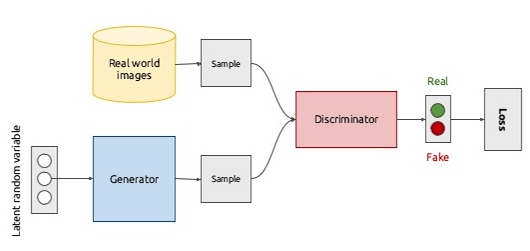
\includegraphics[width=\columnwidth]{GAN_architecture.png}}
    \caption{Architecture of GAN}
    \label{fig:ganarch}
\end{figure}
The Generator model forms data patterns from a latent random variable, which is also simply called noise that is generated in each epoch. The Discriminator model uses data fed into it in order to train, followed by using it to back-propagate to the Generator that uses the feedback from the Discriminator network to get better at producing artificial data of the kind input into the discriminator. The framework explained above is shown in Fig.\ref{fig:ganarch}. This framework of neural networks was first implemented and presented by Ian J. Goodfellow et. Al in 2014\cite{iangan}.
\\
As HPCC Systems was a distributed computing system, there were challenges in implementing Neural Networks in the same. Neural Networks have been implemented in the GNN Bundle described above which uses Tensorflow in the back-end for the Neural Network computations that are needed to be performed. GANs in HPCC Systems were implemented using the GNN bundle by the team working on the same. The paper focuses on how it was implemented along with the results. 

\section{Generalised Neural Networks Bundle (GNN)}\label{gnnsec}

The Generalised Neural Network Bundle, is a bundle that provides a generalised ECL interface to Keras over Tensorflow in Python 3.6. It has various functions that help in the development and usage of Neural Networks very similar to how they would be used in Keras. The documentation for the same has provided on the HPCC Systems website\cite{gnnpaper}.
\\
GNN Bundle utilises the HPCC Systems multi-node processing capability by treating each node on the cluster as a thread of processing which fills the gap between ECL and Python. This makes sure that processing happens in parallel as it should happen in a cluster-computing system. 
\\
Although, the Neural Network model is trained epoch-wise but the processing in each epoch occurs in parallel over the nodes which increases the processing speed when there is a large amount of data that is given as input. 
\\
The bundle is stable for purely Sequential Keras models but is unstable for the Keras Functional models. Due to this, even GANs implemented have a limitation that it purely runs Sequential GAN models of various kinds.
\\
Below are various important modules along with features that have been used widely in the following GAN implementation:

\subsection{The GNNI Module}

GNNI is the main Neural Network module of the GNN bundle. The functions in GNNI are very important when it comes to managing the Neural Network as it doesn't dwell on many details to be given by the user. Given below are features of the following module:

\begin{itemize}
    \item \textbf{Create Session}: Create a Tensorflow session which share global variables for a set of Neural Network models.
    \item \textbf{Define models}: Defines a Sequential Keras model given the Session ID, Definition of each layer as a list of strings and compile definition as a string.
    \item \textbf{Fit data}: Fits the given data to the model.
    \item \textbf{Predict data}: Predicts the output using the model according to input data.
    \item \textbf{Weights transfer}: Retrieving weights from model, storing weights to a JSON file, Input weights from JSON file, Setting weights to a model can all be done with various functions. Helps for saving state of models or transfer between separate but similar models.
    \item \textbf{Evaluation of model}: Evaluation of model to get various metrics or even just getting the previous loss for a fit can be obtained
\end{itemize}

\subsection{The Tensor Module}

For the input of data, Python 3.6 has a numpy package capable of keeping track of the data as an n-dimensional array which is provided as a tensor for handling the input data. For the same framework in ECL, there was a special ECL record structure called $t\_Tensor$ implemented which stores more information than an n-dimensional array while also able to convert to input data for Tensorflow. Given below are the main usable features of Tensor module:

\begin{itemize}
    \item \textbf{Building Tensors}: Tensors may be built from a dataset structured in certain way to build the $t\_Tensor$ dataset fully by using a defined function in this module.
    \item \textbf{Aligning Tensors}: Tensors can be in multiple different lists as per how they are defined. A few functions help in aligning tensors so there isn't a dimension mismatch
    \item \textbf{Get data from Tensor}: The dataset can be extracted from a $t\_Tensor$ using a certain function
    \item \textbf{Miscellaneous features}: Functions to reshape the tensor, add multiple tensors element-wise, get the number of records in a tensor are a few features which could be described as miscellaneous useful features.
\end{itemize}

These features although adequate for basic numerical record, there was a need of much more processing in order to convert a collection images to the required $t\_Tensor$ type. For this, a module was added on to the GNN bundle which is covered in the Section \ref{imagemod}.

\subsection{The Image Module}\label{imagemod}

Processing images to give as input to the Neural Network models developed in GNN is a difficult job due to ECL being a structured language. Defining structure for an image was required along with converting a compressed image format like JPG into a matrix of numbers. After the matrix was obtained, we would need to transform the dataset into a specific structure in order to make the Tensor. Due to these hurdles to process an image, there was a need to make a module which would perform these operations for ease of the user. Given below are the main features that were provided:
\begin{itemize}
    \item \textbf{MNIST dataset}: Functions were implemented to input the images and labels of both train and test datasets of MNIST from the compressed unsigned bytes files obtained online\cite{mnistdat}.
    \item \textbf{Input Image}: The Image that was input in any format was taken as a stream of bytes, then converted into a n-dimensional array in Python using OpenCV 2 functions. This matrix was flattened and then returned along with it's dimensions as a dataset in ECL. To ensure that all images are of the same format, the images are either cropped to certain dimensions in the center or resized to certain dimensions. 
    \item \textbf{Image to Tensor}: The Image was in the form of a list of unsigned integers. This set of numbers was converted to a $t\_Tensor$ as is required for Neural Networks in GNN to take input. 
    \item \textbf{Tensor to Image}: The $t\_Tensor$ which was given from the Neural Network as output was converted into a set of unsigned integers to convert back into an Image for output in various ways.
    \item \textbf{Image output}: The set of Numbers were converted into a numpy matrix and encoded back into an image in JPG or PNG or BMP format for seeing the output. Other than this, a function was implemented to get a collection of images in a grid to see many predictions of generator instead of just one. 
\end{itemize}

\section{Implementation of GAN for HPCC Systems}\label{implementation}

\subsection{Input phase}

The input of data given to the GAN needs to be pre-processed so as to suit the needs of GNN bundle. All the data that is required to be given for training needs to be transformed into a dataset defined as $TensData$ which has the record structure: [indexes, value]. $TensData$ simulates the representation of an n-dimensional array in numpy module with the indexes and value together to represent each position in an array. 
\\
All the data required to be used need to be transformed into the structure of $TensData$ using various transformation operations in ECL. For a dataset that is readily available as CSV or XLS, it is possible to easily transform these. For inputting images into the neural network, the Image module described in Section \ref{imagemod} may be used. It provides straightforward functions to perform the operation described above for input.  

\subsection{Definition of models}

Generative Adversarial Networks by the definition are required to have 2 neural network models, namely the Generator and the Discriminator acting as adversaries to each other. 
\\
Here, the models are required to be given by the user. The user decides on the Generator and Discriminator model definitions and adds definition of each layer into a set of strings. Each model also has a compile definition which is typically a string containing the compile function. Both the models usually must have just one compile definition together. Examples for these are in Section \ref{examples}.
\\
Given these definitions, Generator and Discriminator are defined using the GNNI function $DefineModel(..)$. Along with this, a combined model which is the Generator stacked over the Discriminator needs to be defined. Definition of this combined model is done by appending Generator layer definitions with Discriminator layer definitions, with each layer in discriminator set to non-trainable. This is defined using the same compile definition as the two models. 

\subsection{Training phase}

Each epoch of GAN training happens in the following stages:

\begin{enumerate}
    \item Generate data from random latent variable using Generator.
    \item Fit real data with the label 1 to Discriminator.
    \item Fit generated data with the label 0 to Discriminator.
    \item Fit random latent variable with the label 1 to Combined model. Since Discriminator is non-trainable, Generator is trained with random latent variable while fitting as per Discriminator weights.
\end{enumerate}

Here, the modified weights from Discriminator needs to be transferred to the combined model so that the Fitting of the data to Discriminator is effective in the Epoch. Along with this, the trained weights of the Combined model need to be given to the Generator to predict from noise. If this isn't done, the training of the previous epoch is rendered useless.
\\
In Keras API of Python 3.6, it is possible to make the Combined model by adding the Generator and Discriminator as objects which link their layer weights. In ECL, we need to manually transfer weights to simulate this. 
\\
For this, a weights transfer mechanism was implemented using $GetWeights(..)$ and $SetWeights(..)$ functions in GNNI module of GNN bundle. Figure \ref{wtstran} explains the weights transfer methodology for an $n^{th}$ epoch:

\begin{figure}[htbp]
    \centerline{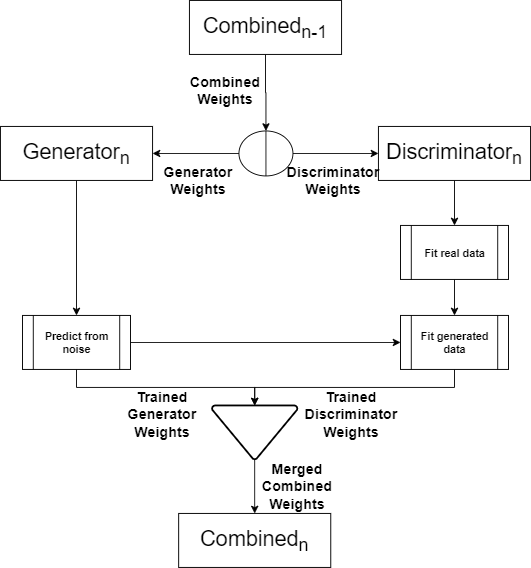
\includegraphics[width=9 cm]{wts_transfer.png}}
    \caption{Weights transfer methodology}
    \label{wtstran}
\end{figure}

\subsection{Output phase}

After the epoch-wise training of the GAN model is performed, both the Generator and Discriminator models are returned from the Module. These models can both be given their respective inputs for checking the output or for an application. 

\subsubsection{\textbf{Generator model}}

Generator model takes an input of a random latent variable, and if required, multiple sets of the random variable to predict data. These predictions are obtained as a $t\_Tensor$, whose data can be extracted using the $GetData(..)$ function in Tensor module. The extracted data can be stored or output to understand the Generator's performance. For an output of images, the Image module in GNN bundle contains functions to easily output the images as is required by the user. 

\subsubsection{\textbf{Discriminator model}}

Discriminator model takes an input of data to classify them as fake or real data. This capability of the Discriminator helps in applications where fraudulent data are to be detected when the number of fraudulent cases are smaller. Machine learning evaluation metrics like AUC, F1 score etc. can be performed on the output dataset with expected to see how the Discriminator has performed.

\section{Choice of dataset for testing}

When working on any model which is used to detect features on an image, MNIST dataset is commonly used. As many may refer to it, the MNIST dataset is the "Hello World" of Deep learning as it is a rather straight forward dataset with minimal noise and clear distinction. It is also said commonly, \begin{quote}
    \textit{If it does not work on MNIST, it will not work at all.}
\end{quote}

Even though that may not be completely true, it is still a great dataset to check the working of most Neural Network implementations. MNIST dataset was initially used by Yann LeCun in his paper about deep learning titled "Gradient based learning applied to document recognition"\cite{lecunmnist}. This dataset is a very simplistic dataset which has handwritten numbers in white with a black background of an uniform size of 28x28 pixels. This enables it to be easily computed and enables neural networks to greatly understand features of the images. 
\\
Classification performed on these numbers with a convolutional neural network enabled the models to get accuracy of upto 99.8\%\cite{mnistdetect}. Due to it being such a good dataset for Neural Networks to use, it works great for us to test GANs on MNIST. Other than these reasons, Ian J. Goodfellow et. Al on their paper titled "Generative adversarial networks", tested their GAN model on MNIST as well\cite{iangan}.

\section{Tested GAN models}\label{examples}

There were two prominent models in GAN which were Sequential in nature for pure generation of data. The output of the generated dataset were checked after subsequent epochs to verify the training that was performed, which are shown in Section \ref{results}. These models were obtained from a github repository called "Keras-GAN" by Erik Linder Noren\cite{kerasgan}.
\\
The Generator and Discriminator models of these are described as follows:

\subsection{Simple Dense layer based Generative Adversarial Networks}

This model is described as a GAN architecture with purely dense based networks with no special transformations except for Batch Normalisation, Dropout and Activation layers. This model tries to see pattern in the image as a whole set by predicting each pixel as per the Dense layer weights obtained after each training epoch. 
\\
The Generator and Discriminator models of the Simple GAN can be seen in Figure \ref{fig:gan_mod}.

\begin{figure*}
     \centering
     \begin{subfigure}[b]{\columnwidth}
         \centering
         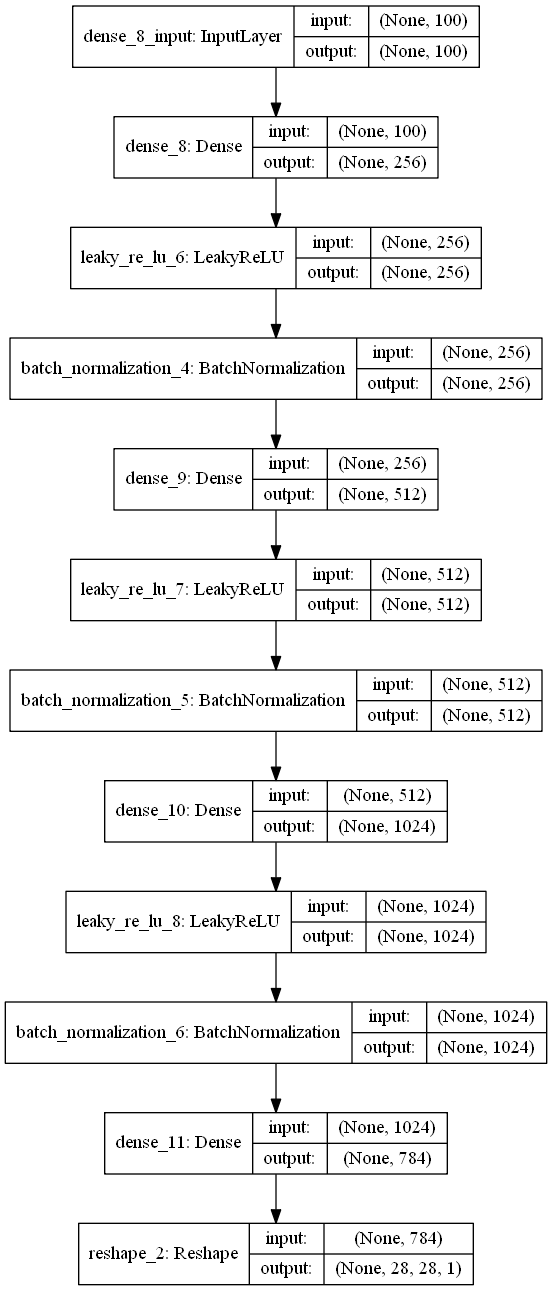
\includegraphics[width=\linewidth]{generator_gan.png}
         \caption{Generator model}
         \label{fig:gen_gan}
     \end{subfigure}
     \hfill
     \begin{subfigure}[b]{\columnwidth}
         \centering
         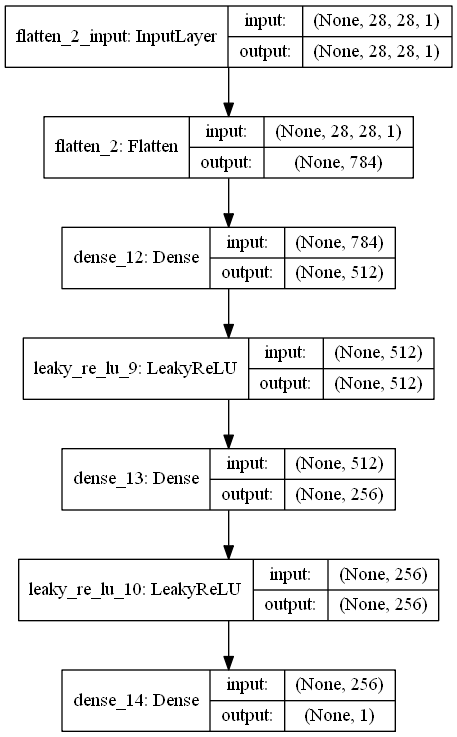
\includegraphics[width=\linewidth]{discriminator_gan.png}
         \caption{Discriminator model}
         \label{fig:dis_gan}
     \end{subfigure}
        \caption{Simple Dense layer based Generative Adversarial Networks}
        \label{fig:gan_mod}
\end{figure*}

As can be seen in Figures \ref{fig:gen_gan} and \ref{fig:dis_gan}, the network consists of purely Dense based models for data manipulation which enables the GAN to be trained pixel-wise. Due to this, the training is much slower than it's other counterparts and the generated images aren't smooth, due to the pixels generated being different. The output of the following model can be seen in Section \ref{gan_results}.
The results in the next model, Deep Convolutional Generative Adversarial Networks (Section \ref{dcgan}), abbreviated as DCGAN, can be seen to provide smoother images compared to Simple GAN. 

\subsection{Deep Convolutional Generative Adversarial Networks}\label{dcgan}

This model is described as a GAN architecture with convolutional transformations in the Neural Network. This model consists of multiple convolutional layers which helps the models in recognizing various features in the image. 
\\
The Generator and Discriminator models of the Deep Convolutional GAN can be seen in Figure \ref{fig:dcgan_mod}.

\begin{figure*}
     \centering
     \begin{subfigure}[b]{\columnwidth}
         \centering
         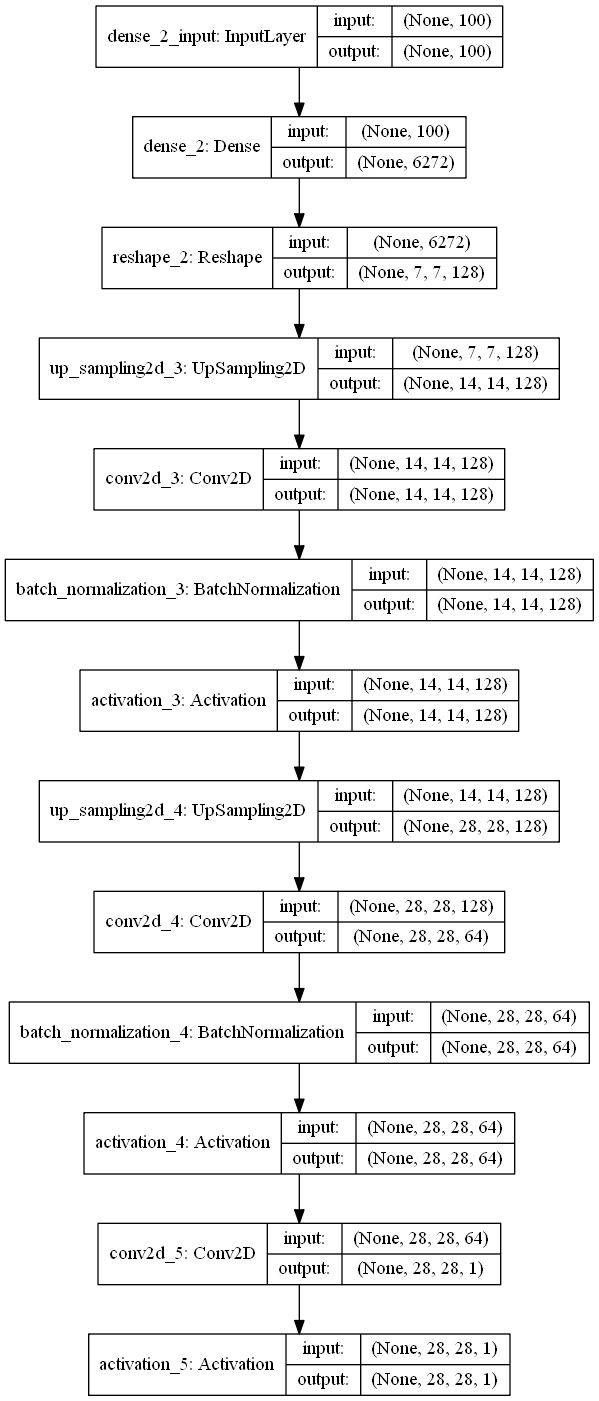
\includegraphics[width=\textwidth,height=\textheight,keepaspectratio]{generator_dcgan.png}
         \caption{Generator model}
         \label{fig:gen_dcgan}
     \end{subfigure}
     \hfill
     \begin{subfigure}[b]{\columnwidth}
         \centering
         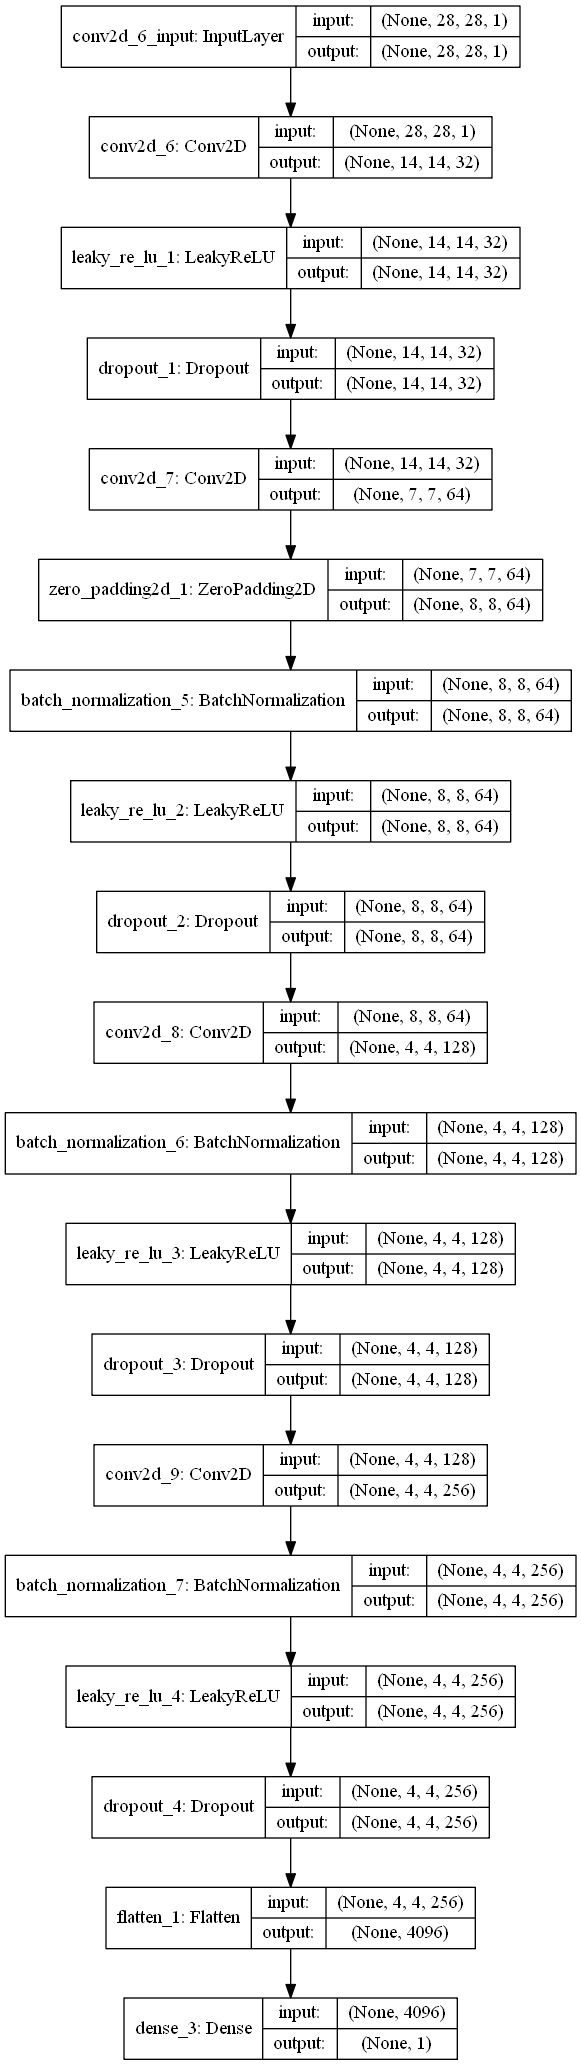
\includegraphics[width=\textwidth,height=\textheight,keepaspectratio]{discriminator_dcgan.png}
         \caption{Discriminator model}
         \label{fig:dis_dcgan}
     \end{subfigure}
        \caption{Deep Convolutional Generative Adversarial Networks}
        \label{fig:dcgan_mod}
\end{figure*}

As can be seen in Figures \ref{fig:gen_dcgan} and \ref{fig:dis_dcgan}, the network consists of convolutional layers along with Dropout layers which increases the feature recognition capability of the network. Due to the improved feature recognition capability, the generated images are much smoother and more unique in nature. The outputs of the following model can be seen in Section \ref{dcgan_results}. It can be observed that DCGAN gives smoother and more unique images as compared to Simple GAN. 

\section{Few notable features}

In the GAN bundle that was implemented for ECL\cite{ganbund}, there are a few features that were implemented which are worth having a discussion about:

\subsection{Saving of trained models}\label{savetrain}

A record structure made to store details of the Generator and Discriminator after being trained in order to fit more data over the trained network or predict to get more snapshots. 
\\
The record structure has the following details: 
\\
    \textbf{Layer specifications} : [Layer definitions, Compile Definition],
        \textbf{Model Weights},\\
        \textbf{Command to despray images},\\
        \textbf{Rows in output grid image},\\
        \textbf{Columns in output grid image},\\
        \textbf{Batch Size to produce noise},\\
        \textbf{Latent dimensions for Random latent variable},\\
        \textbf{Number of epochs for storing in string}
\\
\\
Doing this helps to not lose the model trained and reuse it for various purposes so that the time spent in training isn't deemed worthless. It also helps to experiment over it as and when required after the training is done. 
\\
In $Test/GANtest.ecl$ and $Test/DCGANTest.ecl$, the models are automatically saved at the end so that the user can experiment with the saved model as per their convenience. $Test/SaveTest.ecl$ contains the code snippet of how to save a model, this can be taken as inspiration for using anywhere else.

\subsection{Prediction of models}

The saved model after training as described in Subsection \ref{savetrain} helps for the user to Predict for the model saved as required.
\\
This helps in getting new snapshots of the data by the Generator or to test the Discriminator's distinguishing capabilities on various datasets as required due to a saved model. 
\\
An example of how this works is provided in the $Test/PredictTest.ecl$ file in the GAN bundle. This helps to understand how to use the feature. 

\FloatBarrier
\section{Results}\label{results}

Using the above implementation, two architectures of GANs that were described in Section \ref{examples} have been tested on HPCC Systems using the GAN implementation and executed. Snapshots of the Generator predictions were taken after 2000, 3000 and 4000 epochs respectively, which shows us how the model gets better as it's trained. The outputs of the architectures are as follows:

\subsection{Simple Generative Adversarial Networks}\label{gan_results}

\begin{figure}[htbp]
    \centering
     \begin{subfigure}[b]{\columnwidth}
         \centering
         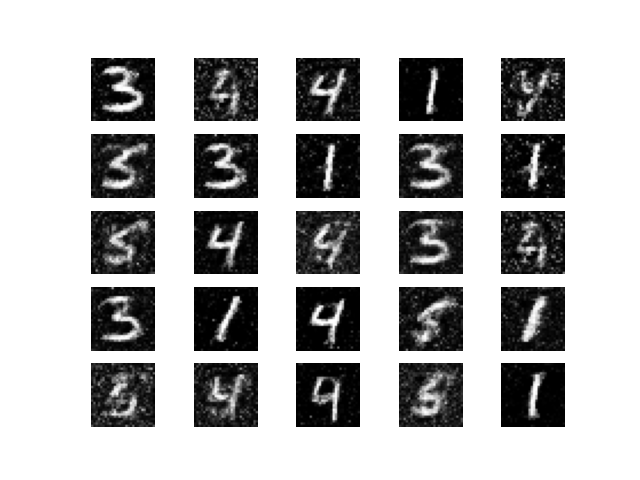
\includegraphics[width=\textwidth,keepaspectratio]{GAN_2000.png}
         \caption{Epoch 2000}
         \label{fig:gan2000}
     \end{subfigure}
     \begin{subfigure}[b]{\columnwidth}
         \centering
         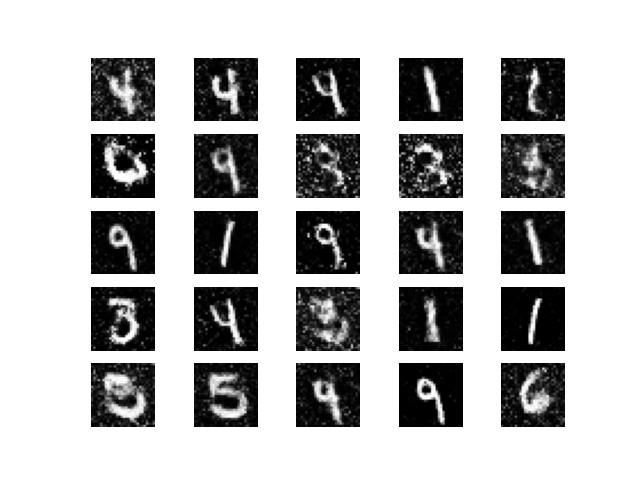
\includegraphics[width=\textwidth,keepaspectratio]{GAN_3000.png}
         \caption{Epoch 3000}
         \label{fig:gan3000}
     \end{subfigure}
     \begin{subfigure}[b]{\columnwidth}
         \centering
         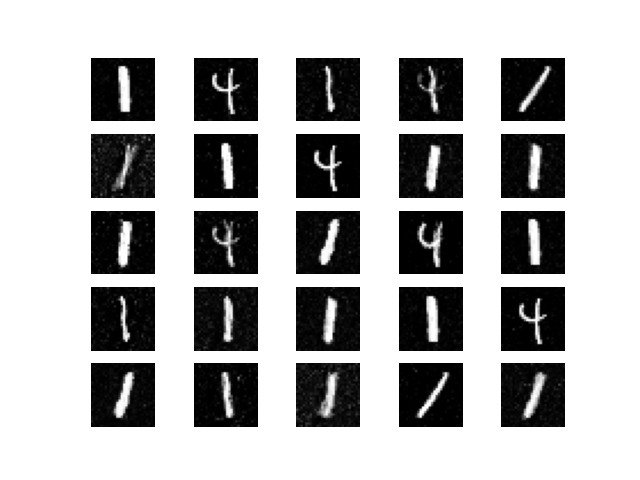
\includegraphics[width=\textwidth,keepaspectratio]{GAN_4000.png}
         \caption{Epoch 4000}
         \label{fig:gan4000}
     \end{subfigure}
        \caption{Generated images from Simple GAN}
        \label{fig:gan_out}
\end{figure}

It can be noticed that Simple GAN produces results very similar to the MNIST dataset, but there are noisy pixels around them due it being a purely dense network relying on the density of each tensor. This is rectified by Deep Convolutional GAN which produces smoother images, with very unique images as compared to Simple GAN.

\subsection{Deep Convolutional Generative Adversarial Networks}\label{dcgan_results}

\begin{figure}[htbp]
    \centering
     \begin{subfigure}[b]{\columnwidth}
         \centering
         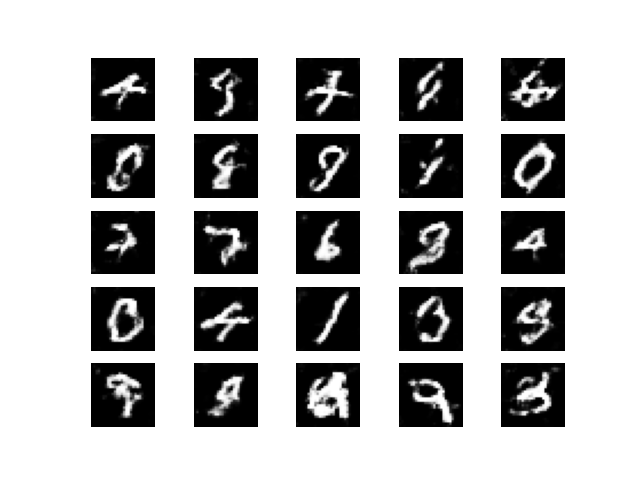
\includegraphics[width=\textwidth,keepaspectratio]{DCGAN_2000.png}
         \caption{Epoch 2000}
         \label{fig:dcgan2000}
     \end{subfigure}
     \begin{subfigure}[b]{\columnwidth}
         \centering
         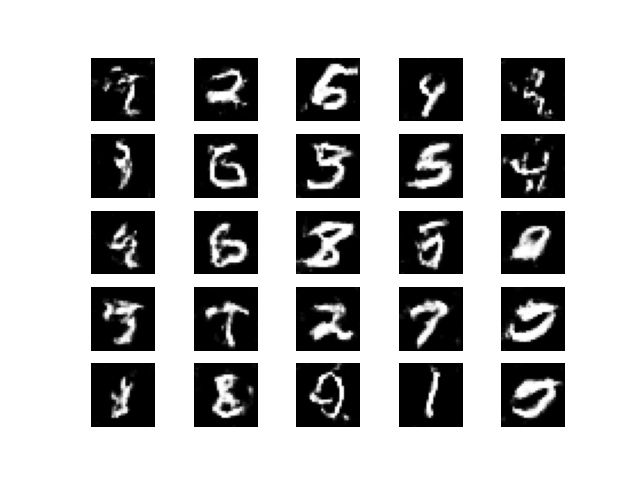
\includegraphics[width=\textwidth,keepaspectratio]{DCGAN_3000.png}
         \caption{Epoch 3000}
         \label{fig:dcgan3000}
     \end{subfigure}
     \begin{subfigure}[b]{\columnwidth}
         \centering
         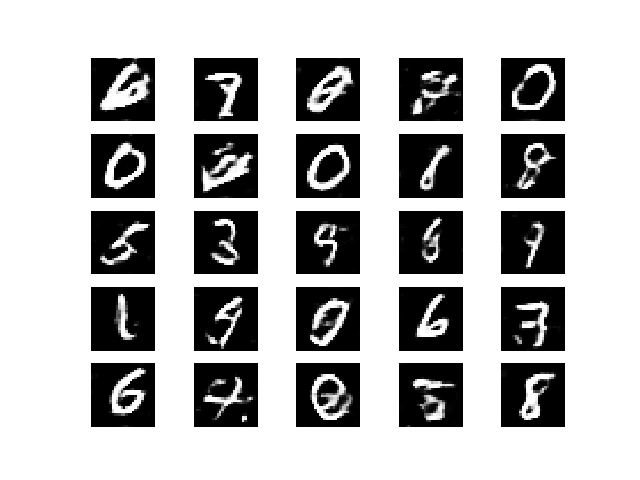
\includegraphics[width=\textwidth,keepaspectratio]{DCGAN_4000.png}
         \caption{Epoch 4000}
         \label{fig:dcgan4000}
     \end{subfigure}
        \caption{Generated images from Deep Convolutional GAN}
        \label{fig:dcgan_out}
\end{figure}

The images produced by Deep Convolutional GAN are much more smoother and unique in nature compared to simple GAN. The convolutional layers implemented in the model detect various features of the MNIST dataset in order to put them together to generate similar digits. The digits generated by both the GAN models get better with more number of training epochs for the GAN.  

\section{Conclusion}

Generative Adversarial Networks were successfully implemented on the HPCC Systems Platform to be able to execute any Keras Sequential GAN model. The implementation has been stable for the models tested on the platform. 
\\
This implementation was made into an ECL bundle to be installed on any system containing the required dependencies. The GAN bundle so created depends on $ML\_Core$ and $GNN$ bundles. So, to use the following implementation, these dependencies need to be installed on the platform. 

\section{Future enhancements}

The implementation for GAN in HPCC Systems has much room for improvement with many more features possible with the proposed architecture above. 
\\
As mentioned above, this implementation of GAN works for purely Sequential models which eliminates the possibility of multiple inputs or outputs as is required for a few types of GAN models. So, an architecture for GAN could be implemented using a GNN Neural Network model similar to the Keras Functional Model API. 
\\
There is quite a confusion for the user as to how the combined model looks like in case the user runs into an error while using the GAN module. Visualising neural network models so as to understand the model better would be very useful.
\\
The debugging of the GAN module could be strange as the error which is logged isn't usually the cause of the error. Improving these debugging prospects of GAN to efficiently track the issue so the user can fix errors would reduce the time taken by the user in solving an error.


\begin{thebibliography}{00}
    \bibitem{abouthpcc} HPCC Systems, "About HPCC Systems", 2020, [Online] Available:
    \url{https://hpccsystems.com/about}. [Accessed July 1, 2020]
    \bibitem{eclguide} HPCC System, "ECL Language Reference", 2020, [Online] Available: \url{https://d2wulyp08c6njk.cloudfront.net/releases/CE-Candidate-7.8.24/docs/EN_US/ECLLanguageReference_EN_US-7.8.24-1.pdf} . [Accessed July 1, 2020]
    \bibitem{mlcore} HPCC Systems, "ML Core Bundle source code", 2020, [Online] Available:
    \url{https://www.github.com/hpcc-systems/ML_Core}. [Accessed July 1, 2020]
    \bibitem{gnn} HPCC Systems, "Generalised Neural Networks Bundle source code", 2020, [Online] Available: 
    \url{https://www.github.com/hpcc-systems/GNN}. [Accessed July 1, 2020]
    \bibitem{iangan} Goodfellow, I.J., Pouget-Abadie, J., Mirza, M., Xu, B., Warde-Farley, D., Ozair, S., Courville, A.C., \& Bengio, Y. (2014). Generative Adversarial Networks. ArXiv, abs/1406.2661.
    \bibitem{gnnpaper} HPCC Systems, "Generalised Neural Networks Bundle documentation", 2020, [Online] Available: \url{https://d2wulyp08c6njk.cloudfront.net/pdf/ml/GNN.pdf}. [Accessed July 11, 2020]
    \bibitem{mnistdat} Yann LeCun, "The MNIST database of Handwritten digits", 2020, [Online] Available: \url{http://yann.lecun.com/exdb/mnist/}. [Accessed July 12, 2020]
    \bibitem{lecunmnist} 	Y. LeCun, L. Bottou, Y. Bengio and P. Haffner: Gradient-Based Learning Applied to Document Recognition, Proceedings of the IEEE, 86(11):2278-2324, November 1998.
    \bibitem{mnistdetect} Baldominos, A., Saez, Y., \& Isasi, P. (2019). A Survey of Handwritten Character Recognition with MNIST and EMNIST. Applied Sciences, 9(15), 3169. doi:10.3390/app9153169.
    \bibitem{kerasgan} Erik Linder Noren, Github, "Keras-GAN", 2020. [Online] Available:
    \url{https://github.com/eriklindernoren/Keras-GAN}. [Accessed July 12, 2020]
    \bibitem{ganbund} Ambu Karthik, Github, "GAN", 2020, [Online] Available:
    \url{https://github.com/dragonfist453/GAN}. [Accessed July 12, 2020]
\end{thebibliography}

\end{document}